\documentclass[runningheads]{llncs}
\usepackage{graphicx}
\usepackage[title]{appendix}
\usepackage{tabularx}

\begin{document}
	\title{CS31620 Vocabulary App - Project Report}
	\author{Rhys Evans}
	\institute{Department of Computer Science, \\ Aberystwyth University, \\ Aberystwyth\\
	\email{rhe24@aber.ac.uk}}
	\maketitle
	
	\begin{abstract}
		The basis of this project was to design and create an Android app to help users learn a new language vocabulary. The App I created is named 'Language Vocabulary Assistant', or 'LVA' in short. The key features of the app are: Specifying a primary and secondary language, storing words or phrases in a viewable list, testing knowledge of the stored words or phrases through practice, and reviewing performance in practices.
	\end{abstract}
	
	\newpage
	\section{Design}
	This section will discuss all aspects of the App's design, this includes both the user interface design and architectural design.  
	\subsection{Architectural Design}
	\subsubsection{Program Flow}
	The app implements an event-driven model, based mostly on user interaction. Most operations are invoked as a direct result of user interaction, therefore the majority of the app's operations are done in the UI thread. Because of this, the classes that do most of the heavy lifting are the Activity and Fragment classes, with the most important class being LVAMainActivity. This is the main activity and entry point of the app, and for the most part remains active throughout the app's lifecycle. The other two activities within the app are LVASetupActivity and PracticeActivity, together, these three activities encapsulate the individual features of the app well and guide program flow. The 'Setup' Activity handles language preference input, whilst the 'Main' activity handles the vocabulary entries and practice stats overview. The 'Practice' activity is dedicated to the quiz-style practice.
	
	\subsubsection{Data Persistence}
	Data is persisted in two ways within the app: shared preferences and a backend SQLite database (see Fig.~\ref{schema}). The user's language selections are stored in the shared preferences, whereas, the SQLite database stores all vocabulary entries and practice attempts. The database interfaces with the SQLite API using the Room Persistence Library. Therefore, for each entity, there needs to be an entity class, a data access object class, and a view-model class. The vocabulary entries entity encapsulates an entry in the vocabulary list, therefore it stores the word/phrase in the primary language and its translation in the secondary language. The practice attempt entity encapsulates an individual practice attempt, this enables the user to view their practice statistics and track performance. The practice attempt entity stores the date of a given attempt, the score achieved and the maximum score of the attempt. 
	
	\newpage
	
	\begin{figure}
		\centering
		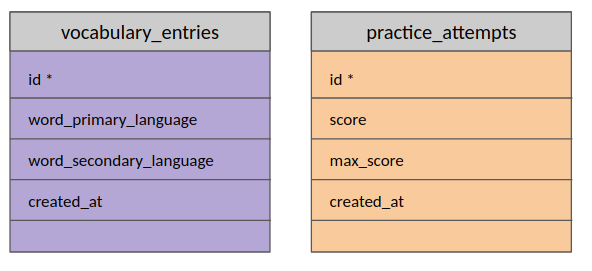
\includegraphics[width=0.75\textwidth]{./img/schema.png}
		\caption{The schema of the SQLite database}
		\label{schema}
	\end{figure}
	
	\subsection{User Interface Design}
	The app's UI design attempts to conform to the principles laid out in google's material design guidelines~\cite{ref_material_design}, using a tab layout and viewpager in the main activity encourages the idea of motion and coherent transformations. Dialogs (see fig.~\ref{dialog}) are used to display important information as their layer of depth imply importance and urgency. Dialogs are especially useful because they do not take the user away from the underlying view, but rather put it on pause whilst an action is required.
	
	The app's color scheme (see Fig.~\ref{styleguide}) was chosen using google's color picker tool~\cite{ref_color_tool}, the color scheme of the app uses a primary color with a light and dark variant and a secondary color used to style accents. Having variance in colour allows separation between important UI elements and layout surfaces. The use of material design icons and android layouts in the app help provide an intuitive affordance, the most prominent example of this is the floating action button on the main activity. A conscious effort was made to use constraint layouts and weighted linear-layouts wherever possible to implement a responsive design. String resources and locale-dependent date formats were also used wherever possible to improve support for localization.
	
	\begin{figure}
		\centering
		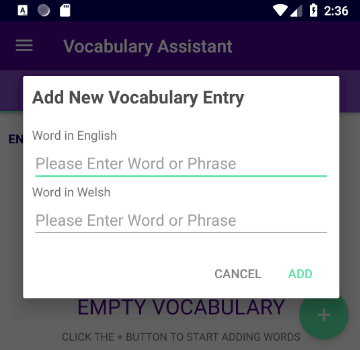
\includegraphics[width=0.5\textwidth]{./img/dialog.png}
		\caption{The 'add new entry' dialog}
		\label{dialog}
	\end{figure}
	
	\newpage
	
	\begin{figure}
		\centering
		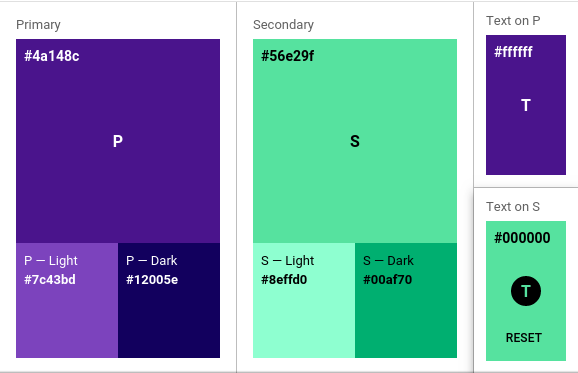
\includegraphics[width=0.75\textwidth]{./img/styleguide.png}
		\caption{The app's styleguide}
		\label{styleguide}
	\end{figure}
	
	\section{Testing}
	In order to effectively test the app and ensure quality, a test table was created. Whenever a new feature was added a test would be designed to ensure it performed as expected. After implementation, each feature was manually tested on two separate devices according to the criteria laid out in the test table (see Table.~\ref{test_table}). After all features were fully implemented and had been manually tested, unit tests and UI tests were created to replace the manual tests for some features. As an improvement for future projects it would be very beneficial if the unit/UI tests were created at the same time as the test table entry is created, thus eliminating the need for labour-intensive manual testing. This could be achieved by refactoring the codebase early on to accommodate things like in-memory databases and Espresso-friendly views. Using unit/UI tests from the beginning would also improve support for regression testing to ensure reliability throughout the program when a new feature is added.
	
	\section{Implementation Review}
	In this section I will review how the implementation of each of the system's key features went, describing any problems encountered during implementation.
	\subsection{Selecting Language Preferences}
	After creating the skeleton layout for the application, this was the first feature that was implemented. A separate activity was created to behave as a 'setup' screen, where the user had two language inputs and a submit button. The first version of this screen used dropdowns to allow the user to make their language selections, the dropdowns were populated from android's vast list of locales. However, as the language selection's only use was to categorize the vocabulary entries and provide a custom display to the user I felt it was appropriate to allow the user to input their own language as a string. This does not limit the user's language selection and they can even store vocabularies for fictional languages, or languages not included in android's locale list. Although the language input field is an edit text view that the user can enter anything into there is an auto-complete popup that appears to recommend languages from the Android locale list to the user. I felt that this simple addition improved user experience considerably and was very simple to implement.
	
	Overall I feel that implementing the setup screen and allowing the user to select their language preferences was fairly straightforward. Once the decision was made to store the selections in the Shared Preferences, it was trivial to force the setup screen on first time launch by checking if any language preferences were already present. A potential improvement for the setup screen is to support a landscape orientation, as currently, the setup screen is the only one that enforces a portrait orientation.
	\subsection{Viewing and Managing The Vocabulary List}\label{ref_vocab_list}
	The vocabulary list fragment contains all things to do with viewing and managing the vocabulary list. To start with I created the XML layout for the overall list and the individual entries. Once the layouts were complete, the model and room database were created. To do this I followed the order of operations laid out in the workbooks, by creating the entity class for a Vocabulary Entry and adding the needed room tags. I then created the data access object and view model class for the vocabulary entry. The most difficult part of this section was to create and debug the room database itself, it was a learning curve to understand what each of the room classes' purpose was and how to handle the Live Data. Once the database was implemented and a recycler view adapter was added for the vocabulary list it was functioning fully and all the backend support for adding and deleting vocabulary entries was in place.
	
	The final task was to implement a user interface for adding, deleting and updating vocabulary entries. For adding and updating entries I opted to implement a custom alert dialog, as per my UI prototypes. Although that I feel this is the approach that provides the best user experience, it was one of the most time consuming tasks in the whole project. Implementing the custom dialog for adding a new entry was fairly trivial, so was adding input validation and backend database support. However, as the 'edit entry' dialog had to be opened from the recycler view's view holder in order to work for each individual entry it provided many unforeseen problems. Whenever the 'edit entry' dialog was opened from the recycler view an 'InvalidStateException' would crash the app. Several attempts were made to fix this issue, including manually managing the fragment transactions for the alert, allowing invalid states in the app and even opening the dialog from an independent 'dialog manager' class. Unfortunately, however, none of these solutions worked, I eventually decided to scrap support for editing entries. Although this was certainly not ideal, I felt there were more critical features to implement and that the vocabulary entries were simple enough that deleting and re-creating them wouldn't be too laborious for the user. For future projects I would either use an entirely separate activity, thus circumventing the need for fragment transactions or I would adapt the design such that, the recycler view's view holder never had to execute any UI tasks and simply passed information about the vocabulary entry to some dialog manager class.
	
	Although not specified in the requirements, I added a sort button to the vocabulary list, allowing the user to sort by created date (ascending and descending) and alphabetically (ascending and descending). This was surprsisingly simple to implement and only required the addition of a few extra SQL queries in the repository, DAO, and view-model classes.
	\subsection{View Performance in Practices}
	The second tab in the main activity's tab layout is the practice overview. From here the user can see a breakdown of their performance in practices, they can also start a new practice attempt. The most time intensive aspect of this feature was providing backend support for storing data about each practice attempt. Although the process was very similar to that of persisting vocabulary entries, it required a database migration to add the new table. However, once this was done the rest of the implementation went smoothly, for the presentation of all the statistics, I deviated from my prototype and opted for a circular progress indicator and to display scores as a percentage. An unforeseen issue with the 'out of 10' display I had specified in my prototypes was that not all practices would have a maximum score of 10. Therefore the 'average score' display would not work correctly. Making this change was fairly straightforward, I simply had to store the maximum score for each practice attempt and work out the percentage on creation of the fragment.
	\subsection{Practicing}
	Along with the vocabulary list, this is one of the most important features in the system, therefore it took some time to get right. Creating the recycler list was very similar to the one created for~\ref{ref_vocab_list}, with minor changes to the individual entries' layout to accommodate an edit text. The one key difference between this recycler view of vocabulary entries and the main list is that the 'setHasFixedSize' and 'setItemViewCacheSize' attributes are used in the practice list. Although this is typically considered bad practice for a recycler view as it technically defeats their purpose, however, s the recycler view to display practice questions always has a fixed size, this isn't necessarily a major issue. It was the simplest solution to an issue where the contents of a list item's edit text were being replicated several times through the list.
	
	One major challenge when implementing this feature was to ensure that the chosen sample of entries would remain the same throughout a practice. As the sample of entries is chosen in the activity's 'onCreate' method, there was a danger that it would be reset to a whole new sample every time the screen was rotated. Therefore the list of entries, along with the user's input for each entry needed to be stored in the activity's instance state. This required some changes to the Vocabulary Entry and Practice Answer classes in order to make them parcelable so they could be stored in the instance state bundle.
	
	\section{Conclusion}
	Overall, I believe that I have created an aesthetically pleasing app that conforms to android's material design principles. I feel that the user interface is very intuitive and allows the user to use/access every feature in the application with ease. With the exception of updating/editing a vocabulary entry I feel that my app fully implements all of the required features outlined in the assignment specification and provides some extra functionality that could be considered flair. One notable shortcoming of the app is the lack of multiple practice formats, the app currently only supports a 'question-answer' format of vocabulary practice. I felt this was the most realistic implementation given the time-frame, if future updates were made to the app, this would certainly be on the top of the list. As mentioned in the testing section, I feel that I created a very comprehensive test plan for manual testing. But could have done with creating more unit and UI tests sooner in the development process.
	
	Taking all of the above into account, I feel that the project deserves a reasonably high mark. The app meets all of the requirements laid out, I created a reasonably thorough and reliable test plan and followed the core design principles from the workshops. As mentioned in the above sections there are some shortcomings within the app that should be considered. For example, no support for updating vocabulary entries, only one practice format, UI testing certainly has room for improvement. I hope that these have been sufficiently addressed within this report.
	 
	\begin{thebibliography}{10}
		\bibitem{ref_material_design}
		Material Design. (2018). Introduction. [online] Available at: https://material.io/design/introduction/\# [Accessed 5 Dec. 2018].
		\bibitem{ref_color_tool}
		Color Tool - Material Design. (2018). Color Tool - Material Design. [online] Available at: https://material.io/tools/color/\#!/?view.left=0\&view.right=0 [Accessed 5 Dec. 2018].
		
	\end{thebibliography}
	
	\begin{subappendices}
		\renewcommand{\thesection}{\Alph{section}}
		
		\section{Features}
		\begin{itemize}
			\item \textbf{FR1} - If no language preferences are present, show user the setup screen.
			\item \textbf{FR2} - Allow user to input and submit two language preferences that are then saved to shared preferences.
			\item \textbf{FR3} - Assist user input with language auto complete
			\item \textbf{FR4} - Ensure language selections are valid.
			\item \textbf{FR5} - Allow user to change language preferences, the user should be prompted with a confirmation dialog.
			\item \textbf{FR6} - Changing the language preferences deletes the current vocabulary list and practice statistics.
			\item \textbf{FR7} - User should be able to delete their current vocabulary list, a confirmation dialog should show.
			\item \textbf{FR8} - Allow user to create a new vocabulary entry by inputting word/phrase in both languages. System should handle validation for user input.
			\item \textbf{FR9} - User should be able to view a scrollable list of all their vocabulary entries
			\item \textbf{FR10} - User should be able to delete a given vocabulary entry, this action should be 'undo-able'
			\item \textbf{FR11} - User should be able to sort the vocabulary entries list by date created and alphabetically.
			\item \textbf{FR12} - User should be able to view the time/date of their last practice attempt
			\item \textbf{FR13} - User should be able to view the score of their last practice
			\item \textbf{FR14} - User should be able to view their best practice score
			\item \textbf{FR15} - User should be able to view their average practice score
			\item \textbf{FR16} - User should be able to start a new practice attempt
			\item \textbf{FR17} - When a practice attempt is started, the user should be presented with 10 random entries from their vocabulary list, if they don't have 10 entries it should show all of their entries.
			\item \textbf{FR18} - The 10 random entries in the practice list should show the word in primary language and provide an input box for the user to type in the word in the secondary language.
			\item \textbf{FR19} - Allow the user to abandon a current practice attempt by either pressing an on-screen button or their phone's physical back button. User should be prompted for confirmation first.
			\item \textbf{FR20} - Allow the user to submit the practice at any time, this will open a dialog displaying their results
			\item \textbf{FR21} - The dialog should display the user's score for the practice.
			\item \textbf{FR22} - If the user had incorrect answers, show them the corrections.
			\item \textbf{FR23} - Allow the user to dismiss the results dialog and return back to main activity.
		\end{itemize}
		
		\section{Test Table}
		\begin{table}
			\caption{The app's test table that covers all implemented features}\label{test_table}
			\begin{tabularx}{\textwidth}{|l|X|X|X|X|l|}
				\hline
				\textbf{ID} & \textbf{Requirement} & \textbf{Description} & \textbf{Input} & \textbf{Output} & \textbf{PASS/FAIL} \\
				\hline
				001 & FR1 & Verify that when app is launched without any preferences saved, the user is sent to setup screen. & Start app without any preferences saved & Setup screen is displayed & PASS \\
				\hline
				002 & FR2 & Check that language preferences can be inputted and saved & Type valid preferences into language input fields and press submit & Preferences are saved into database & PASS \\
				\hline
				003 & FR3 & Check that language input autocomplete is working & Start typing into language input fields & After two characters are entered, a popup appears with language suggestions & PASS \\
				\hline
				004 & FR4 & Check that input validation for language preference is working correctly & Provide invalid input as language preference and submit & Error message shows & PASS \\
				\hline
				005 & FR5 & Check that language preferences can be changed & Press 'change language' button and confirm the dialog & Current preferences are deleted & PASS \\
				\hline
				006 & FR6 & Check that changing language preferences also deletes vocabulary list and practice stats & Change the language preferences whilst there are entries in the vocabulary list & Vocabulary list and practice overview stats are be empty & PASS \\
				\hline
				007 & FR7 & Check that vocabulary list can be deleted & Press the 'delete vocabulary list' option and confirm dialog & Vocabulary list table is emptied along with all associated practice stats & PASS \\
				\hline
				008 & FR8 & Check that 'add new vocabulary entry' button works  & Press the 'add new entry' button & A dialog with inputs is shown  & PASS \\
				\hline
				009 & FR8 & Check that new vocabulary entries are properly created & Press the 'add new entry' button and input new word & New entry is saved to database & PASS \\
				\hline
				010 & FR8 & Verify that input validation for new vocabulary entry works & Submit an invalid word entry to new vocabulary entry dialog & Error message is displayed and word is not added to vocab list & PASS \\
				\hline
			\end{tabularx}
		\end{table}
		
		\newpage
		
		\begin{table}
			\begin{tabularx}{\textwidth}{|l|X|X|X|X|l|}
				\hline
				011 & FR9 & All vocabulary entries should be displayed in a scrollable list & Naviagte to 'vocabulary list' tab and scroll through entries & All entries are present and displayed properly & PASS \\
				\hline
				012 & FR10 & Check that vocabulary entries can be deleted & Press the 'delete' button on a given entry and confirm dialog & Entry is no longer in the database & PASS \\
				\hline
				013 & FR10 & Check that deleted vocabulary entries can be retrieved via 'undo' & Delete a vocabulary entry and press 'undo' on the snackbar & The deleted entry is re-added into the database & PASS \\
				\hline
				014 & FR11 & Check that vocabulary list can be sorted & Press the 'sort' button and sort the list by the different criteria & The list has changed order correctly depending on sorting criteria & PASS \\
				\hline
				015 & FR12 & Check that the user can view the date and time of their last practice & Navigate to 'practice overview' tab & Correct date and time of last practice attempt is be displayed & PASS \\
				\hline
				016 & FR13 & Check that the user can view their most recent practice score & Navigate to 'practice overview' & Correct score for most recent practice is dispalayed & PASS \\
				\hline
				017 & FR14 & Check that user can view their best practice score & Navigate to 'practice-overview' & Correct best score is displayed & PASS \\
				\hline
				018 & FR15 & Check that user can view their average pratice score & Navigate to 'practice-overview' & Correect average score is displayed & PASS \\
				\hline
				019 & FR16 & Check that user can start a new practice attempt & Press 'start new practice' button & A new practice activity is shon & PASS \\
				\hline
				020 & FR17 & Check that correct number of vocabulary entries are displayed in practice list & Start a new practice & atleast 10 entries are displayed & PASS \\
				\hline
				021 & FR18 & Check that the user can enter answers to practice questions & Start a new practice & Answer inputs are displayed by each vocabulary entry & PASS \\
				\hline
			\end{tabularx}
		\end{table}
		
		\newpage
		
		\begin{table}
			\begin{tabularx}{\textwidth}{|l|X|X|X|X|l|}
				\hline
				022 & FR19 & Check that current practice can be abandoned & Press the 'abandon' button or physical back button and confirm dialog & The practice activity is closed & PASS \\
				\hline
				023 & FR20 & Check that practice can be submitted & Press the 'submit' button & Results dialog is opened & PASS \\
				\hline
				024 & FR21 & Check that user is shown their score after practice submission & Submit a practice & Score is shown on dialog & PASS \\
				\hline
				025 & FR22 & Check that incorrect answers are shown on results dialog & Submit a practice with incorrect answers & Incorrect answers and corrections are shown & PASS \\
				\hline
				026 & FR23 & Check that results dialog can be dismissed & Dismiss the results dialog & Practice activity closes & PASS \\
				\hline 
			\end{tabularx}
		\end{table}
	\end{subappendices}
\end{document}